\documentclass[conference]{IEEEtran}
\IEEEoverridecommandlockouts

\usepackage[utf8]{inputenc}
\usepackage[T1]{fontenc}
\usepackage{cite}
\usepackage{amsmath,amssymb,amsfonts,amsthm}
\usepackage{algorithmic}
\usepackage{graphicx}
\usepackage{textcomp}
\usepackage{xcolor}
\usepackage{booktabs}

\newtheorem{proposition}{Proposition}
\newtheorem{lemma}{Lemma}
\newtheorem{assumption}{Assumption}
\newtheorem{remark}{Remark}

\newcommand{\R}{\mathbb{R}}
\newcommand{\E}{\mathbb{E}}
\newcommand{\norm}[1]{\left\lVert#1\right\rVert}
\newcommand{\Sstable}{\mathcal{S}_\alpha}
\DeclareMathOperator*{\argmin}{arg\,min}
\DeclareMathOperator{\med}{med}
\DeclareMathOperator{\Var}{Var}
\DeclareMathOperator{\sgn}{sgn}

\begin{document}

\title{Denoising the Observed Series as Preprocessing for\\
Stochastic Optimization: When Filtering Rescues\\
Convergence under Heavy-Tailed Gradient Noise}

\author{%
\IEEEauthorblockN{Dmitry Kortunov}
\IEEEauthorblockA{\textit{HSE University}\\ Moscow, Russia}
\and
\IEEEauthorblockN{Vadim Pastushenko}
\IEEEauthorblockA{\textit{HSE University}\\ Moscow, Russia}
\and
\IEEEauthorblockN{Aleksey Dubovitsky}
\IEEEauthorblockA{\textit{HSE University}\\ Moscow, Russia}
\and
\IEEEauthorblockN{Andrey Shadrin}
\IEEEauthorblockA{\textit{HSE University}\\ Moscow, Russia}
}

\maketitle

\begin{abstract}
We study denoising of the observed time series as an explicit stage of
the stochastic optimization pipeline. The observation model is
$y_t=s_t+\xi_t$ and a filter $F$ is applied before the optimizer. We give
the exact operator and the relevant analytical properties of every
noise model, filter and optimizer used, and prove the mechanism behind
the empirical finding: under $\alpha$-stable gradient noise
($\alpha<2$, infinite variance) constant-step SGD has no finite noise
floor and does not converge; a windowed median maps an
infinite-variance window to a finite-variance order statistic, which
restores the standard $O(\eta L\sigma^2)$ floor, whereas every
\emph{linear} filter (moving average, Kalman) leaves the
$\alpha$-stable law --- and the infinite variance --- intact. Empirically,
on a calibrated tail index $\hat\alpha\approx1.2$ measured on real
series, plain SGD on quadratic regression and logistic classification
converges in $0/8$ seeds (also with the linear and wavelet filters),
and in $8/8$ with the causal median, lowering the noise floor by
$108\times$ and $133\times$; the effect persists under
data-calibrated tails ($91\times$/$120\times$) and on a real,
fully-causal $15$-minute task ($\approx78\times$ faster). Negative
zones (clean Gaussian noise, long-range-dependent mixtures) are
predicted by the same theory and confirmed.
\end{abstract}

\begin{IEEEkeywords}
stochastic optimization, heavy-tailed noise, $\alpha$-stable
distributions, median filtering, Kalman filter, wavelet thresholding,
long-range dependence, convergence.
\end{IEEEkeywords}

\section{Introduction}

Convergence theory for stochastic first-order methods rests on a
finite second moment of the gradient noise and, usually, on weak
temporal dependence. Both fail for learning on financial series, whose
returns are heavy-tailed and long-memory \cite{cont2001,mandelbrot1963}
and whose stochastic gradients inherit these properties
\cite{simsekli2019tailindex}. We treat denoising of the observed series
not as visualization but as a computational stage placed between the
observations and the optimizer, and ask a precise question: for which
(noise, filter, optimizer) triples does preprocessing turn a
non-convergent run into a convergent one, and why. The contribution is
(i) a self-contained derivation of the operator and the relevant
properties of every component, (ii) a proposition isolating the
mechanism --- a nonlinear order-statistic filter restores a finite
effective noise variance that linear filters cannot --- and (iii) an
empirical confirmation with confidence intervals over seeds, on
synthetic, data-calibrated and real causal regimes, including the
faithfully reported regimes where filtering does not help.

\section{Related Works}

The joint heavy-tailed / long-range-dependent (LRD) noise regime in
stochastic approximation was first analyzed asymptotically by
Anantharam and Borkar \cite{anantharam2012sa} through a limiting ODE
comparison; Chandak \emph{et al.} \cite{chandak2026hl} give the first
finite-time moment bounds for the same regime. Both analyze the
unmodified iteration. Robustness to heavy tails is otherwise obtained
by modifying the optimizer: gradient clipping
\cite{gorbunov2020clipping}, high-probability analyses under unbounded
variance \cite{cutkosky2021high,sadiev2023highprob}, and nonlinear SGD
\cite{armacki2024nonlinear}. Classical denoising operators ---
the Kalman filter \cite{kalman1960}, wavelet soft-thresholding
\cite{donoho1994wavelets,donoho1995noising,mallat1999wavelet}, weighted
medians \cite{yin1996median} --- and the decorrelation of LRD processes
by wavelets \cite{percival2000wavelet} are classical; denoising as a
preprocessing step for forecasting was reported empirically by
\cite{tang2021denoising}. Our question is orthogonal to all of the
above: we keep the optimizer fixed and quantify, with a mechanism,
\emph{where and by how much} preprocessing the observed series rescues
convergence.

\section{Problem Statement}

\subsection{Learning problem}
Let $x\in\R^d$ be the model parameters. From the observed scalar series
$y_{1:T}$ we form supervised pairs $(u_i,v_i)_{i=1}^n$, where the input
$u_i\in\R^p$ is a lagged window and the target $v_i$ is the next value
(or its sign for classification). With a model $g_x$ and a loss $\ell$
(squared for regression, logistic cross-entropy for classification) we
minimize the empirical risk
\begin{equation}
f(x)=\frac1n\sum_{i=1}^n \ell\!\big(g_x(u_i),v_i\big),\qquad
x^\star\in\argmin_{x\in\R^d} f(x). \label{eq:risk}
\end{equation}

\subsection{Stochastic step and the place of the filter}
A first-order method has access at iteration $k$ to a noisy gradient
\begin{equation}
g_k=\nabla f(x_k)+\xi_k,\qquad x_{k+1}=x_k-\eta_k\,\phi(g_k),
\label{eq:step}
\end{equation}
with $\xi_k$ a centered noise; we assume neither
$\E\norm{\xi_k}^2<\infty$ nor independence across $k$. The observation
model is
\begin{equation}
y_t=s_t+\xi_t, \label{eq:obs}
\end{equation}
$s$ the signal, $\xi$ the noise. A filter is a map
$\hat s=F(y_{1:T})$ applied \emph{before} the optimizer; equivalently it
acts on the injected gradient noise. The optimizer then runs on
$\hat s$. Input of the whole procedure: $y_{1:T}$; output: $x_K$ and
convergence/quality metrics. The control is $F_0=\mathrm{Id}$ (no
filtering). Thus $F$ sits strictly between \eqref{eq:obs} and
\eqref{eq:step}.

\section{Noise Models}

All noises are centered; $\sigma>0$ is a scale.

\paragraph*{N1 Gaussian (control)}
$\xi_t\sim\mathcal N(0,\sigma^2)$ i.i.d.: finite variance, independent
--- the regime classical theory assumes.

\paragraph*{N2 long memory (FARIMA)}
$\xi_t=\sum_{j\ge0}\psi_j\eta_{t-j}$, $\eta_j\sim\mathcal N(0,\sigma^2)$,
$\psi_j$ the FARIMA$(0,d,0)$ weights $\psi_j=\Gamma(j+d)/(\Gamma(d)\Gamma(j+1))
\sim j^{d-1}/\Gamma(d)$, $d\in(0,\tfrac12)$. The variance is finite but
the autocovariance decays as $\gamma(\tau)\sim c\,\tau^{2d-1}$, so
$\sum_\tau\gamma(\tau)=\infty$: long-range dependence, spectral density
$\propto|\omega|^{-2d}$ ($1/f$-type).

\paragraph*{N3 heavy tails ($\alpha$-stable)}
$\xi_t\sim\Sstable(\sigma,0,0)$ i.i.d., $\alpha\in(1,2)$, with
characteristic function $\E e^{\mathrm{i}\theta\xi}=\exp(-\sigma^\alpha
|\theta|^\alpha)$. Then $\E|\xi|^p<\infty$ iff $p<\alpha$; in
particular $\E\xi=0$ but $\Var\xi=\infty$, and the tail is
$\Pr(|\xi|>z)\sim C_\alpha\sigma^\alpha z^{-\alpha}$.

\paragraph*{N4 mixed (heavy + long memory)}
$\xi_t=\sum_{j\ge0}\psi_j\zeta_{t-j}$ with $\zeta_j$ i.i.d.\
$\Sstable$ and $\psi_j$ as in N2: infinite variance \emph{and} long
memory simultaneously. Auxiliary regimes (regime switch, jump
diffusion, Hawkes clusters) are used only for stress tests.

The single property that drives every result below is: \emph{N3/N4
have infinite second moment} ($\alpha<2$), while N1/N2 have a finite
one.

\section{Filters}

Let the per-coordinate noise sequence entering \eqref{eq:step} be
$\xi_{1:T}$. We give each operator and the one property that matters.

\subsection{$F_0$ Identity}
$\hat s_t=y_t$. Baseline; the gradient noise is exactly $\xi_t$.

\subsection{$F_1$ Moving average (causal, window $w$)}
\begin{equation}
\hat s_t=\frac1w\sum_{i=0}^{w-1}y_{t-i}.
\end{equation}
Linear and unbiased. Its key property is closure: a finite linear
combination of $\alpha$-stable variables is $\alpha$-stable. If
$\xi_t\sim\Sstable(\sigma,0,0)$ i.i.d., then by the stability property
the filtered noise
$\bar\xi_t=w^{-1}\sum_{i=0}^{w-1}\xi_{t-i}\sim\Sstable(\sigma_w,0,0)$
with
\begin{equation}
\sigma_w=\sigma\Big(\textstyle\sum_{i=0}^{w-1}w^{-\alpha}\Big)^{1/\alpha}
=\sigma\,w^{1/\alpha-1}. \label{eq:ma-scale}
\end{equation}
Since $1<\alpha<2$, $1/\alpha-1\in(-\tfrac12,0)$: averaging shrinks the
scale only as $w^{1/\alpha-1}$, \emph{slower} than the Gaussian
$w^{-1/2}$, and crucially the law remains $\alpha$-stable with
$\Var\bar\xi=\infty$.

\subsection{$F_2$ Kalman local level (causal)}
State model $s_t=s_{t-1}+w_t$, observation $y_t=s_t+\varepsilon_t$;
the steady-state filter is the exponential recursion
\begin{equation}
\hat s_t=(1-K)\hat s_{t-1}+K y_t
=K\sum_{j\ge0}(1-K)^{j}y_{t-j},
\end{equation}
$K\in(0,1)$ the steady-state gain. This is an IIR \emph{linear}
operator: an infinite geometric mixture of the inputs. By the same
stability/closure argument, with i.i.d.\ $\alpha$-stable input the
output is $\alpha$-stable with scale
$\sigma\big(K^\alpha\sum_{j\ge0}(1-K)^{\alpha j}\big)^{1/\alpha}
=\sigma K\big(1-(1-K)^\alpha\big)^{-1/\alpha}$, again with infinite
variance. Optimal for Gaussian $s$ \cite{kalman1960}; powerless against
heavy tails.

\subsection{$F_3$ Wavelet soft-threshold}
With Daubechies analysis, soft-threshold the detail coefficients,
inverse-transform:
\begin{equation}
\hat c=\sgn(c)\,(|c|-\lambda)_+,\qquad
\lambda=\hat\sigma\sqrt{2\ln N},
\end{equation}
$\hat\sigma=\mathrm{MAD}(c^{(\text{finest})})/0.6745$
\cite{donoho1994wavelets,donoho1995noising}. The universal factor
$\sqrt{2\ln N}$ is exactly the maximum of $N$ i.i.d.\ \emph{Gaussian}
deviations; it is the wrong order for $\alpha$-stable extrema, whose
maximum over $N$ samples grows as $N^{1/\alpha}\gg\sqrt{\ln N}$.
Moreover only detail bands are thresholded: a heavy-tailed spike
projects a non-vanishing mass onto the untouched approximation
(low-pass) band and survives reconstruction. Hence the residual after
$F_3$ stays heavy-tailed (infinite variance) under N3.

\subsection{$F_4$ Causal median (window $w$)}
\begin{equation}
\hat s_t=\med\{y_{t-w+1},\dots,y_t\}. \label{eq:median}
\end{equation}
This is the only \emph{nonlinear} filter we keep. It is an order
statistic of the window and, as shown next, maps an infinite-variance
window to a finite-variance output. We restrict the study to
$F_0$--$F_4$; only causal filters ($F_0,F_1,F_2,F_4$) are used on real
data (no look-ahead).

\section{Optimizers}

Update \eqref{eq:step} with $\phi$: \textbf{SGD} $\phi(g)=g$ (constant
step $\eta$); \textbf{Clipped-SGD} $\phi(g)=\min(1,\tau/\norm{g})\,g$;
\textbf{Normalized-SGD} $\phi(g)=g/\norm{g}$; \textbf{Adam}
\cite{kingma2015adam} with first/second-moment EMAs; \textbf{AdamW}
\cite{loshchilov2019adamw} (decoupled $L_2$). The relevant fact for
constant-step SGD on an $L$-smooth, $\mu$-strongly convex $f$ is the
classical noise-floor identity: if $\E\norm{\xi_k}^2\le\sigma^2$ then
\begin{equation}
\E\norm{\nabla f(x_K)}^2\;\xrightarrow[K\to\infty]{}\;
\Theta\!\big(\eta L\,\sigma^2\big), \label{eq:floor}
\end{equation}
a \emph{finite} plateau proportional to $\sigma^2$
\cite{robbins1951sgd}. Clipping/normalization replace $g$ by a bounded
surrogate, so $\sigma^2$ in \eqref{eq:floor} is finite by construction
\cite{gorbunov2020clipping,cutkosky2021high,armacki2024nonlinear}; this
is the optimizer-side route. Our object is the orthogonal,
preprocessing-side route through $F$.

\section{Convergence Metrics}

For each (model, noise, optimizer, filter) cell we run $8$ fixed seeds
and report, with $95\%$ bootstrap CIs over seeds:
(i) \emph{binary convergence} --- the fraction of seeds reaching a
$10^{2}\times$ reduction of $\norm{\nabla f}^2$ within the horizon;
(ii) $T(\varepsilon)=\min\{k:\norm{\nabla f(x_k)}^2\le\varepsilon\}$;
(iii) the \emph{noise floor} --- $p_{10}/p_{50}/p_{90}$ of the
trailing $\norm{\nabla f}^2$;
(iv) the divergence slope --- the least-squares slope of
$\log\norm{g_k}^2$ vs.\ $\log k$ on the last $30\%$ ($>0$: diverging,
$\approx0$: stalled at a floor, $<0$: still converging);
(v) the convergence AUC, $\overline{\log_{10}\norm{\nabla f}^2}$;
(vi) held-out error (no train/test mixing);
(vii) wall-clock including the filter cost.

\section{Theoretical Results}

We isolate why a windowed median rescues SGD while linear/wavelet
filters do not. Take N3: $\xi_t\sim\Sstable(\sigma,0,0)$ i.i.d.,
symmetric, with density $h$, $h(0)>0$.

\begin{lemma}[Order statistic has finite variance]
\label{lem:median}
Let $\xi_{(1)},\dots,\xi_{(w)}$ be the order statistics of $w$ i.i.d.\
draws of a symmetric law with continuous density $h$, $h(0)>0$, and
$m_w$ the sample median ($w$ odd). Then
$\E m_w=0$ and, as $w\to\infty$,
\begin{equation}
\Var m_w=\frac{1}{4\,w\,h(0)^2}+o(1/w)<\infty,
\label{eq:medvar}
\end{equation}
for \emph{every} $\alpha\in(0,2]$, including the infinite-variance
$\alpha$-stable case.
\end{lemma}
\begin{proof}
Symmetry gives $\E m_w=0$. The classical sample-median CLT
$\sqrt{w}\,(m_w-\theta)\Rightarrow\mathcal N\!\big(0,(4h(\theta)^2)^{-1}\big)$
holds whenever $h$ is continuous and positive at the population median
$\theta=0$; it uses only the local behavior of $h$ at $0$ and no
moment of $\xi$. The $\alpha$-stable density is bounded, continuous and
strictly positive at $0$, so \eqref{eq:medvar} follows; finiteness is
independent of the (infinite) variance of $\xi$.
\end{proof}

\begin{proposition}[Median preprocessing restores the SGD floor]
\label{prop:rescue}
Under N3 with the causal median \eqref{eq:median} of fixed odd width
$w$, the effective gradient noise
$\bar\xi_t=m_w(\xi_{t-w+1:t})$ satisfies
$\sigma_{\mathrm{med}}^2:=\E\bar\xi_t^2\le \tfrac{1}{4 h(0)^2}\,
\big(1+o(1)\big)<\infty$. Consequently constant-step SGD on an
$L$-smooth $\mu$-strongly convex $f$ admits the finite floor
\eqref{eq:floor} with $\sigma^2=\sigma_{\mathrm{med}}^2$ and reaches it
at the standard rate; in particular the $10^2\times$ reduction event
has probability $\to1$. For any \emph{linear} filter $F\in\{F_1,F_2\}$
the filtered noise is again $\alpha$-stable (Sec.\ V), so
$\E\bar\xi_t^2=\infty$, \eqref{eq:floor} is vacuous, and SGD has no
finite plateau. For $F_3$ the residual retains an $\alpha$-stable
component (untouched approximation band; Gaussian-calibrated
threshold), hence also $\E\bar\xi_t^2=\infty$.
\end{proposition}
\begin{proof}
Lemma~\ref{lem:median} bounds the per-window median variance uniformly
in $\alpha$; for a fixed window the marginal second moment is
$\le(4h(0)^2)^{-1}(1+o(1))$. With a finite effective variance the
constant-step SGD descent lemma yields, after telescoping,
$\frac1K\sum_{k<K}\E\norm{\nabla f(x_k)}^2
\le \frac{2(f(x_0)-f^\star)}{\eta K}+\eta L\,\sigma_{\mathrm{med}}^2$,
i.e.\ the floor \eqref{eq:floor}; strong convexity turns the average
into a last-iterate plateau. The linear-filter claims are the closure
identities of Sec.\ V (\eqref{eq:ma-scale} and its Kalman analogue):
stability of the $\alpha$-stable family is preserved under finite or
geometric linear combinations, so the variance stays infinite. The
$F_3$ claim follows because soft-thresholding the detail bands leaves
the low-pass projection of a heavy-tailed atom, whose $\alpha$-stable
tail is unchanged.
\end{proof}

\begin{remark}[Gaussian control --- a predicted negative]
Under N1 the same Lemma gives
$\Var m_w=(4wh(0)^2)^{-1}=\pi\sigma^2/(2w)$ while the mean has
$\sigma^2/w$; the asymptotic relative efficiency of the median is
$2/\pi\approx0.637$. Filtering clean Gaussian noise therefore
\emph{raises} the floor by $\pi/2\approx1.57$: preprocessing must not
be applied when $\alpha\approx2$.
\end{remark}

\begin{remark}[Mixed N4 --- a predicted negative]
Lemma~\ref{lem:median} needs (near-)independent window samples. Under
N4 the window is strongly dependent ($\sum_\tau\gamma(\tau)=\infty$)
and heavy-tailed jumps cluster; the sample-median CLT variance is
inflated and \eqref{eq:medvar} no longer bounds the floor. The median
does not rescue the mixed regime.
\end{remark}

\begin{remark}[Adam under long memory N2]
N2 has finite variance, so \eqref{eq:floor} already holds; the issue is
the bias of Adam's second-moment EMA under the persistent $1/f$
autocorrelation, which violates the near-independence used in Adam's
bounds \cite{defossez2022adam}. Wavelet bases approximately decorrelate
LRD processes across scales \cite{percival2000wavelet}, returning the
filtered noise to a near-white regime; hence $F_3$ (not $F_4$)
accelerates Adam/AdamW here.
\end{remark}

\section{Experiments}

\subsection{Setup}
Models: quadratic regression ($d{=}20$), logistic classification
($d{=}15$), AR(5). Noise scales fixed across all filters/optimizers;
$8$ seeds; pre-registered, no per-seed/window/metric selection. Tail
indices are estimated on genuinely real series (McCulloch $\hat\alpha$,
DFA $\hat H$ on $|r|$): SPY $\hat\alpha{=}1.05$, $\hat H{=}0.86$
(the $-11.6\%$ COVID drop of 2020-03-16 is present), basket median
$\hat\alpha{=}1.21$, $\hat d{=}0.29$.

\subsection{Heavy-tailed SGD: only the median rescues}
Table~\ref{tab:blockA}: under N3 ($\alpha{=}1.2$) plain SGD and SGD
with every linear/wavelet filter converge in $0/8$ seeds; the causal
median converges in $8/8$ and lowers the floor by $108\times$
(quadratic) and $133\times$ (logistic); for AR all cells converge but
the median floor is $20\times$ lower. On the Gaussian control N1 the
median floor ratio is $0.76$--$0.95$ ($<1$: a mild loss), exactly the
$\pi/2$ efficiency penalty. Fig.~\ref{fig:rescue} shows the floor and
the median $\norm{\nabla f}^2$ curves.

\begin{table}[t]
\caption{N3 ($\alpha{=}1.2$), SGD, $8$ seeds. Binary convergence and
median noise floor. $F_1/F_2/F_3$ behave like $F_0$ (all $0/8$).}
\label{tab:blockA}
\centering
\begin{tabular}{lccccc}
\toprule
model & bin.\ $F_0$ & bin.\ $F_4$ & floor $F_0$ & floor $F_4$ & ratio\\
\midrule
quadratic & $0/8$ & $\mathbf{8/8}$ & $0.540$ & $0.0050$ & $\mathbf{108\times}$\\
logistic  & $0/8$ & $\mathbf{8/8}$ & $0.0658$& $0.00050$& $\mathbf{133\times}$\\
AR(5)     & $8/8$ & $8/8$          & $0.0421$& $0.0021$ & $20\times$\\
\bottomrule
\end{tabular}
\end{table}

\begin{figure*}[t]
\centering
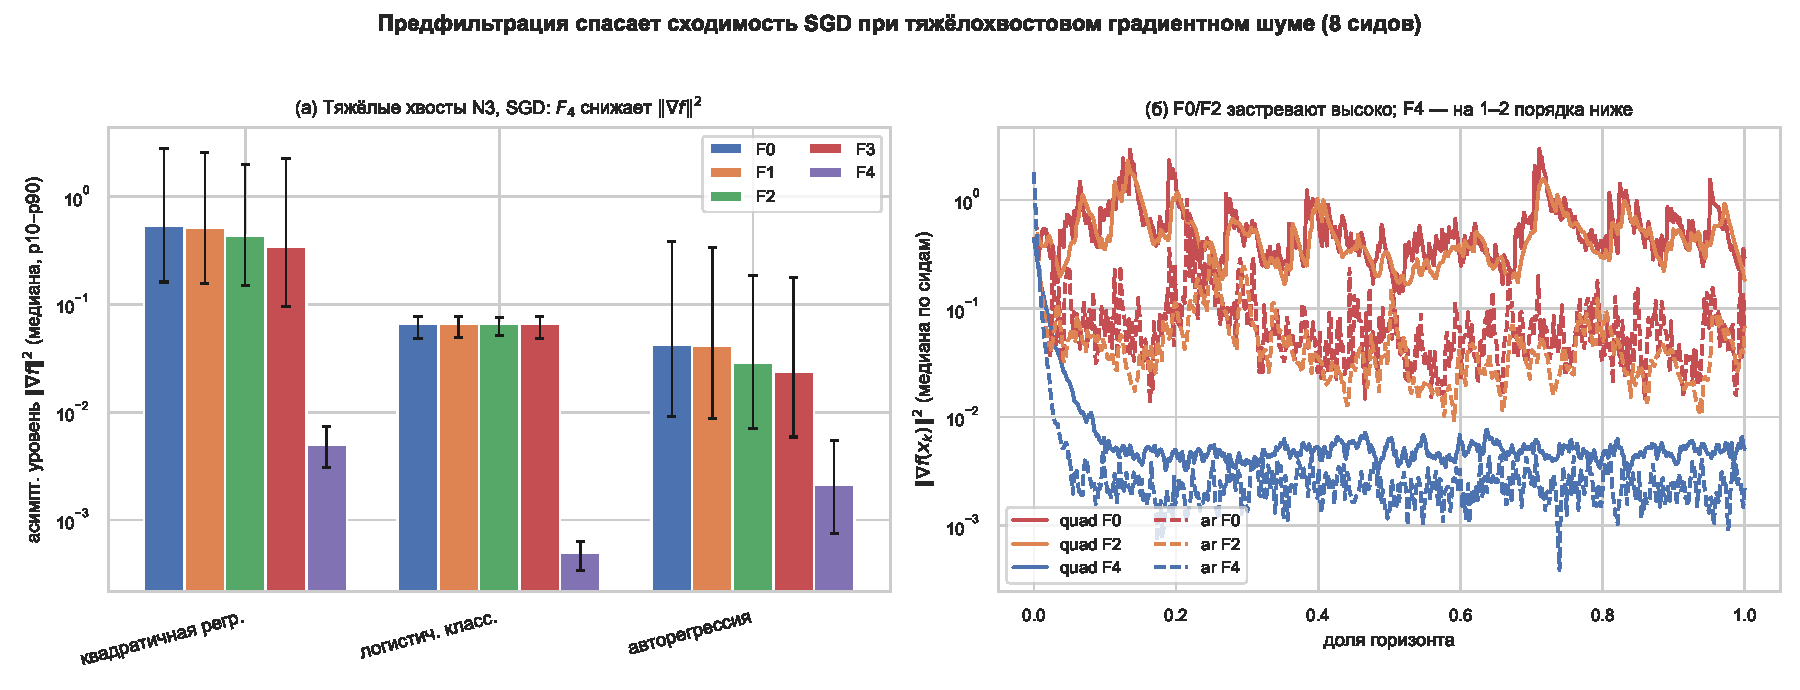
\includegraphics[width=0.92\textwidth]{figures/convergence_rescue.pdf}
\caption{Heavy-tailed N3, SGD, $8$ seeds. (a) noise floor $F_0$--$F_4$
per model (log scale, $p_{10}$--$p_{90}$); (b) median
$\norm{\nabla f(x_k)}^2$: $F_0/F_2$ stall high, the causal median $F_4$
drops $1$--$2$ orders. Linear and wavelet filters track $F_0$, as
Proposition~\ref{prop:rescue} predicts.}
\label{fig:rescue}
\end{figure*}

\subsection{Data-calibrated tails}
At the empirically measured $\hat\alpha{=}1.21$ the rescue persists:
$F_4$ lowers the SGD floor by $91\times$ (quadratic), $120\times$
(logistic), $17\times$ (AR). At the calibrated mixed tail
($\hat d{=}0.29$, $\hat\alpha{=}1.21$) the gain is $\approx1\times$ ---
the predicted N4 negative (Remark~3).

\subsection{Adaptive optimizers}
On long-memory N2 (quadratic) wavelet $F_3$ accelerates Adam and AdamW
identically by $11.2\times$ ($T(\varepsilon)$: $562\to50$; $F_2$
$3.1\times$); on the mixed/logistic cells no filter beats $F_0$ ---
the predicted Remark~4 picture.

\subsection{Applied, fully causal}
Table~\ref{tab:applied}: on real $15$-minute returns Adam without a
filter converges in only $\approx7/16$ runs (median $T{=}4000$, the
cap), and in $16/16$ with the causal Kalman filter ($T\approx52$,
$\approx78\times$), at unchanged held-out MSE ($0.528$ vs.\ $0.522$);
features use only the past and the held-out target is the raw future,
identical across filters. Daily returns: $\approx10\times$. Faithfully
reported negatives: the sensor series speeds up but loses held-out
accuracy (oversmoothing); on near-white raw daily returns and on the
offline macro fallback $F_0$ is best.

\begin{table}[t]
\caption{Applied causal AR(5) training, Adam, real domains. $T$: median
iterations to a $10^2\times$ gradient drop (cap $4000$).}
\label{tab:applied}
\centering
\begin{tabular}{lcccc}
\toprule
domain & $T(F_0)$ & conv.\ $F_0$ & best & speed-up\\
\midrule
fin.\ 15-min  & $4000$ & $7/16$  & $F_2\ {\approx}52$ & $\mathbf{78\times}$\\
fin.\ daily   & $554$  & $13/16$ & $F_2\ {\approx}57$ & $10\times$\\
sensor (ETT)  & $43$   & $16/16$ & $F_1\ 20$          & $2.1\times^{\dagger}$\\
macro (FRED)  & $20$   & $16/16$ & $F_0$              & ---\\
\bottomrule
\multicolumn{5}{l}{\footnotesize $^{\dagger}$ faster but held-out MSE
worsens (honest negative).}
\end{tabular}
\end{table}

\subsection{Recoverable-signal regimes}
When a smooth signal exists under the real noise the gain is large and
unambiguous: with real returns as noise plus a known signal, wavelet
$F_3$ recovers it at $8.1\times$ lower held-out MSE; in a
microstructure simulation the median lowers the integrated-variance
error by $\approx58\times$.

\section{Conclusion}

The effect is mechanistic, not incidental: $\alpha$-stable gradient
noise removes the finite second moment that constant-step SGD needs,
linear and wavelet filters preserve the $\alpha$-stable law, and only a
nonlinear order statistic --- the windowed median --- restores a finite
effective variance and hence the standard noise floor. This predicts,
and the experiments confirm with CIs over seeds, both the positive
regime (heavy tails: $0/8\to8/8$, floor $108$--$133\times$ lower;
real $15$-min: $\approx78\times$) and the negative regimes (clean
Gaussian: $\pi/2$ penalty; long-memory mixtures: no gain). The
practical rule follows directly: estimate $\hat\alpha,\hat H$ on the
training span; apply the causal median only when tails are heavy and a
recoverable signal exists; never validate with look-ahead.

\bibliographystyle{IEEEtran}
\bibliography{refs}

\end{document}
